\title{Domain, Codomain, Range} 
\subtitle{\SubTitleName}
\institute[]{\Course}
\author{\Instructor}
\maketitle   


\frame{\frametitle{Topics and Learning Objectives}
    \Emph{Topics} \\
    \TopicStatement
    \begin{itemize}
        \item the definition of a linear transformation
        \item domain, codomain, image, and range
        \item the interpretation of matrix multiplication as a linear transformation
    \end{itemize}
    
    \vspace{0.5cm}

    \LO\\
    
    \LearningObjectiveStatement

    \begin{itemize}
        % \item Construct and interpret linear transformations in $\mathbb R^n$ (for example, interpret a linear transform as a projection, or as a shear).
        \item characterize linear transforms using the concepts of domain, codomain, image, and range

    \end{itemize}
    



}




\begin{frame}
\frametitle{From Matrices to Functions}

Let $A$ be an $m \times n$ matrix. We define a function
\begin{align*}
T: \R^n &\to \R^m, \quad T(\vec v) = A \vec x
\end{align*}
This is called a \Emph{matrix transformation}.

\begin{itemize}
    \item The \Emph{domain} of $T$ is $\R^n$.

    \item The \Emph{codomain} of $T$ is $\R^m$.

    \item The vector $T(\vec x)$ is the \Emph{image} of $\vec x$ under $T$.
    
    \item The set of all possible images $T(\vec x)$ is the \Emph{range}.

\end{itemize}

% This gives us \Emph{another} interpretation of  $A\vec x = \vec b$:
% \begin{itemize}
%     \item set of equations 
%     \item augmented matrix
%     \item matrix equation
%     \item vector equation 
%     \item linear transformation equation
% \end{itemize}

\end{frame}

\begin{frame}
\frametitle{Functions from Calculus}

    Many of the functions we know have \Emph{domain} and \Emph{codomain} $\R$. We can express the \Emph{rule} that defines the function $\sin$ this way:

    \[ f\colon\R\rightarrow\R \qquad f(x) = \sin(x) \]

    In calculus we often think of a function in terms of its graph. The horizontal axis is the \Emph{domain}, the vertical axis is the \Emph{codomain}.

    \begin{center}
    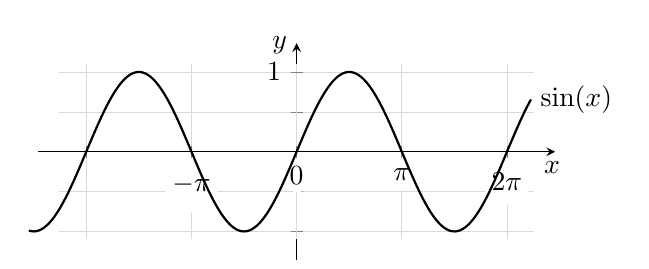
\begin{tikzpicture}[domain=-8:7] 
        \begin{axis}[
        width=3in,
        height=1.5in,
        grid=both,
        grid style={line width=.2pt, draw=gray!30},
        clip=false,
        axis lines=middle,
        xmin=-7.1,xmax=7.1,
        ymin=-1.1,ymax=1.1,
        restrict y to domain=-2:4,
        xtick={-6.28,-3.14,0,3.14,6.28},
        xticklabels={, , , , , , , , , ,},
        ytick={-1,-0.5,0,0.5,1},
        yticklabels={, , , , , , , , , ,},
        extra x ticks={-3.14,0,3.14,6.28},
        extra y ticks={1},
        extra x tick style={xticklabel style={fill=white, circle, inner sep=1.5pt}},
        extra y tick style={xticklabel style={fill=white, circle, inner sep=1.5pt}},
        extra x tick labels={$-\pi$,$0$, $\pi$,$2\pi$},
        extra y tick labels={1},
        axis line style={shorten >=-7.5pt, shorten <=-7.5pt},
        xlabel=$x$,
        ylabel=$y$,
        xlabel style={at={(ticklabel* cs:1)},anchor=north west},
        ylabel style={at={(ticklabel* cs:1)},anchor=south east}
        ]
        \addplot[samples=100,domain=-8:7,smooth, thick] {sin(deg(x))} node[pos=1] (endofplotsquare) {};
        \node [right] at (endofplotsquare) {$\sin(x)$};      
        \end{axis}
    \end{tikzpicture}   
    \end{center}


%   This is ok when the domain and codomain are $\R$. It's hard to do when the domain is $\R^2$ and the codomain is $\R^3$. We would need five dimensions to draw that graph.

\end{frame}






\begin{frame}
\frametitle{Example: A Matrix Transformation}

Let  $A=\begin{pmatrix} 1&1\\0&1\\1&1 \end{pmatrix}, \quad
\vec u=\begin{pmatrix} 3\\4 \end{pmatrix}, \quad
% \vec b=\begin{pmatrix} 7\\5\\7\end{pmatrix}, \quad 
T(\vec x) = A\vec x $\\[12pt]

\begin{enumerate}[a)]

    \item What is the domain and codomain of $T$? \vfill

    \item Compute the image of $\vec u$ under $T$. \vfill
    
    \item What is the range of $T$? \vfill
    
\end{enumerate} 

\end{frame}

\begin{frame}
\frametitle{From Matrices to Functions}

The function
\begin{align*}
T: \R^n &\to \R^m, \quad T(\vec v) = A \vec x
\end{align*}
gives us \Emph{another} interpretation of  $A\vec x = \vec b$. We now have five ways of representing $A\vec x = \vec b$:
\begin{itemize}
    \item set of linear equations 
    \item augmented matrix
    \item matrix equation
    \item vector equation 
    \item linear transformation equation
\end{itemize}

\end{frame}

\begin{frame}


\frametitle{Example: A Matrix Transformation as a System}

Consider again the matrix $A=\begin{pmatrix} 1&1\\0&1\\1&1 \end{pmatrix}$, and associated transform $T(\vec x) = A\vec x $.

\begin{enumerate}[a)]
    
    \item Calculate $\vec v \in \R^2$ so that $T(\vec v)= \vec b =\begin{pmatrix} 7\\5\\7\end{pmatrix}$ \vfill
    \item Give a $\vec c \in \R^3$ so there is no $\vec v$ with $T(\vec v)= \vec c$. \\ 
    or: Give a $\vec c$ that is not in the range of $T$. \\
    or: Give a $\vec c$ that is not in the span of the columns of $A$.

\end{enumerate} 

\end{frame}





\frame{\frametitle{Summary}

\SummaryLine \vspace{4pt}
\begin{itemize}\setlength{\itemsep}{8pt}
        \item Characterized linear transforms using the concepts of domain, codomain, image, and range.
        \item The interpretation of matrix multiplication as a linear transformation. 

\end{itemize}

}


